%% UWAGI
%% - wszystkie pliki kodujemy w utf8
%% - stosujemy biber'a do obsługi bibliografii; nie stosujemy bibtex'a;
%%   Overleaf automatycznie wykrywa biber'a; w innych środowiskach być może
%%   będziesz musiał ustawić go ręcznie
%% - proponujemy pakiet acro do obsługi synonimów; jeśli nie widzisz potrzeby korzystania z synonimów,
%%   to zakomentuj dwie linijki w tym pliku

\documentclass[12pt, a4paper, twoside, titlepage]{report}

%%% Copyright (C) [2026] [PWr * WIT * Wydziałowa Komisja d/s Jakości Kształcenia]
%%% Zmodyfikowany i zoptymalizowany (2026)
%%% ---------------------------------------------------------------------------

%%% KONFIGURACJA EKSTRAKCJI TEKSTU (PDF COPY-PASTE)
\input{glyphtounicode} 
\pdfgentounicode=1     % Wymagane przez JSA (Jednolity System Antyplagiatowy)

%%% 1. KODOWANIE I JĘZYK
\RequirePackage[T1]{fontenc}
%\RequirePackage[utf8]{inputenc} % Opcjonalne w nowych systemach (domyślne)
\RequirePackage[english,polish]{babel} % Kolejność eng -> pl
\RequirePackage{csquotes} % Wymagane przez biblatex

%%% 2. MATEMATYKA I CZCIONKI
%%% WIT / Zasady Grebera: Times New Roman 12 pt w całym dokumencie.
%%% newtx* = nowoczesny klon Times (tekst + matematyka w tej samej rodzinie).
%%% Wyjątek: listingi/kod — \ttfamily (maszynowa), zgodnie z praktyką techniczną.
\RequirePackage{amsmath}
\RequirePackage{mathtools}
\RequirePackage{amsthm}

\RequirePackage{newtxtext}
\RequirePackage{newtxmath}
\RequirePackage{microtype} % Poprawia optyczny wygląd tekstu
\renewcommand{\familydefault}{\rmdefault} % serif wszędzie (bez sffamily na tytule)

%%% 3. GEOMETRIA I GRAFIKA
%%% wymogi_edytorskie: 25 mm + 5 mm na oprawę (lewa / inner)
\RequirePackage{geometry}
\geometry{
  a4paper,
  top=25mm, bottom=25mm,
  inner=25mm, outer=25mm,
  bindingoffset=5mm
}
\RequirePackage{graphicx}
\RequirePackage{xcolor}
\RequirePackage{float} % Dla opcji pozycjonowania [H]

%%% 4. NARZĘDZIA POMOCNICZE
\RequirePackage{etoolbox}
\RequirePackage{indentfirst} % wcięcie także pierwszego akapitu po tytule

%%% 5. FORMATOWANIE TEKSTU I NAGŁÓWKÓW
%%% wymogi_edytorskie: rozdział 14 pt, podrozdział 13 pt, 2. rząd 12 pt; interlinia 1;
%%% Zasady Grebera: justowanie, bez kropek po tytułach rozdziałów
\RequirePackage{titlesec}
\RequirePackage{caption}
\RequirePackage{subcaption}
\RequirePackage{setspace}

\setlength{\parindent}{0.7cm}
\singlespacing % wymogi_edytorskie: interlinia pojedyncza (klasa report justuje tekst)

% Rozmiary WIT (Times / newtx): 14 / 13 / 12 pt
\newcommand{\WitChapterFont}{\normalfont\bfseries\fontsize{14}{17}\selectfont}
\newcommand{\WitSectionFont}{\normalfont\bfseries\fontsize{13}{16}\selectfont}
\newcommand{\WitSubsectionFont}{\normalfont\bfseries\fontsize{12}{14.5}\selectfont}

\titleformat{\chapter}[display]
  {\WitChapterFont}
  {\chaptertitlename\ \thechapter}{0.5ex}
  {\WitChapterFont}
\titlespacing*{\chapter}{0pt}{-20pt}{20pt}

\titleformat{\section}{\WitSectionFont}{\thesection.}{1em}{}
\titlespacing*{\section}{0pt}{2.5ex plus 1ex minus .2ex}{1.3ex plus .2ex}

\titleformat{\subsection}{\WitSubsectionFont}{\thesubsection.}{1em}{}
\titlespacing*{\subsection}{0pt}{2.25ex plus 1ex minus .2ex}{1.0ex plus .2ex}

\titleformat{\subsubsection}{\WitSubsectionFont}{\thesubsubsection.}{1em}{}
\titlespacing*{\subsubsection}{0pt}{2.0ex plus 1ex minus .2ex}{0.8ex plus .2ex}

% Numeracja ciągła wewnątrz rozdziałów (Tabela 2.1 / Rys. 2.1)
\counterwithin{figure}{chapter}
\counterwithin{table}{chapter}
\numberwithin{equation}{chapter}

% Podpisy: 10 pt, ta sama rodzina Times; Greber: „Rys.” / „Tabela”
\renewcommand{\figurename}{Rys.}
\renewcommand{\tablename}{Tabela}
\captionsetup{
  font={small,rm},
  labelfont={bf,rm},
  labelsep=period,
  justification=centering,
  skip=10pt
}

%%% 6. ALGORYTMY I LISTINGI KODU
\RequirePackage{algorithm}
\RequirePackage{algpseudocode}
\algrenewcommand\algorithmiccomment[1]{\hfill\(\triangleright\) #1}
\floatname{algorithm}{Algorytm} 

\RequirePackage{listings}
\definecolor{codebg}{RGB}{250,250,250}
\definecolor{codekw}{RGB}{0,64,160}
\definecolor{codestr}{RGB}{0,128,0}
\definecolor{codecmt}{RGB}{128,128,128}

\lstset{
  basicstyle=\ttfamily\small,
  backgroundcolor=\color{codebg},
  keywordstyle=\bfseries\color{codekw},
  stringstyle=\color{codestr},
  commentstyle=\itshape\color{codecmt},
  numbers=left,
  numberstyle=\tiny\color{gray},
  stepnumber=1,
  numbersep=8pt,
  tabsize=2,
  showstringspaces=false,
  breaklines=true,
  frame=lines,
  captionpos=b,
  % Mapowanie polskich znaków dla listings (niezbędne przy tym pakiecie)
  literate={ą}{{\k{a}}}1 {ć}{{\'c}}1 {ę}{{\k{e}}}1 {ł}{{\l{}}}1 {ń}{{\'n}}1 {ó}{{\'o}}1 {ś}{{\'s}}1 {ż}{{\.z}}1 {ź}{{\'z}}1
           {Ą}{{\k{A}}}1 {Ć}{{\'C}}1 {Ę}{{\k{E}}}1 {Ł}{{\L{}}}1 {Ń}{{\'N}}1 {Ó}{{\'O}}1 {Ś}{{\'S}}1 {Ż}{{\.Z}}1 {Ź}{{\'Z}}1
}
\renewcommand{\lstlistingname}{Listing}
\renewcommand{\lstlistlistingname}{Spis listingów}

% Styl Haskell 
\definecolor{darkgreen}{rgb}{0,0.5,0}
\lstdefinestyle{haskellStyle}{
    language=Haskell,
    commentstyle=\color{darkgreen},
    keywordstyle=\color{blue}\bfseries,
    basicstyle=\ttfamily\small,
    breaklines=true,
    stringstyle=\color{red}
}

%%% 7. HYPERREF I CLEVEREF (Musi być na końcu)
\RequirePackage[
    pdfusetitle,
    colorlinks=true,
    linkcolor=black,
    citecolor=blue,
    urlcolor=blue,
    bookmarksnumbered=true
]{hyperref}

\RequirePackage[nameinlink]{cleveref}

% Tłumaczenia dla cleveref (Greber: „rys.” / pełne „tabela”)
\crefname{figure}{rys.}{rys.}
\Crefname{figure}{Rysunek}{Rysunki}
\crefname{table}{tabela}{tabele}
\Crefname{table}{Tabela}{Tabele}
\crefname{equation}{równ.}{równ.}
\Crefname{equation}{Równanie}{Równania}
\crefname{listing}{listing}{Listingi}
\crefname{algorithm}{algorytm}{algorytmy}
\Crefname{algorithm}{Algorytm}{Algorytmy}

%%%%%%%%%%%
%% MAKRA %%
%%%%%%%%%%%

% Definicja rodzaju pracy 
\newcommand{\stRodzajPracy}{%
  \ifnum\stCzyMgr=1 MAGISTERSKA\else INŻYNIERSKA\fi
}

\newcommand{\StronaTytulowa}{
  \pagenumbering{roman}
  \normalfont % ta sama rodzina Times co reszta pracy (bez sffamily)
  \begin{titlepage}
    \newgeometry{top=2.5cm, bottom=2.5cm, left=2.5cm, right=2.5cm}

    \begin{center}
      {\fontsize{18}{22}\selectfont\bfseries Politechnika Wrocławska \par}
      \vspace{0.4cm}
      {\fontsize{14}{17}\selectfont Wydział Informatyki i Telekomunikacji \par}
    \end{center}
    \par\noindent\rule{\textwidth}{1pt}\par
    \vspace{0.5cm}

    {\normalsize
    \begin{tabular}{@{}ll}
      Kierunek: & \textbf{\stKierunek\ (\stKodKierunku)} \\
      \ifdefempty{\stSpecjalnosc}{}{Specjalność: & \textbf{\stSpecjalnosc\ (\stKodSpecjalnosci)}}
    \end{tabular}
    }

    \vspace*{\fill}

    \begin{center}
      {\fontsize{16}{19}\selectfont\bfseries PRACA DYPLOMOWA \par}
      \vspace{0.3cm}
      {\fontsize{16}{19}\selectfont\bfseries \stRodzajPracy \par}
      \vspace{2.0cm}
      {\fontsize{14}{17}\selectfont\bfseries \stTytulPL \par}
      \vspace{1cm}
      {\fontsize{14}{17}\selectfont \stAutor \par}
      \vspace{2cm}
      {\normalsize Opiekun pracy:\par \textbf{\stOpiekun} \par}
    \end{center}

    \vspace*{\fill}

    {\raggedright
      \small Słowa kluczowe: \textit{\stSlowaKluczowe}\par
      \vspace{0.5em}
      \par\noindent\rule{\textwidth}{1pt}\par
    }

    \begin{center}
      \fontsize{14}{17}\selectfont Wrocław \stRok
    \end{center}

    \restoregeometry
  \end{titlepage}
  \normalfont
  \pagestyle{empty}
}

\newenvironment{abstracts}{}{\selectlanguage{polish}\clearpage}

\newcommand{\AbstractPL}{
  \begin{center}{\WitChapterFont Streszczenie \par}\end{center}\vspace{0.5em}
}

\newcommand{\AbstractENG}{
  \selectlanguage{english}
  \begin{center}{\WitChapterFont Abstract \par}\end{center}\vspace{0.5em}
}

\newcommand{\SpisTresci}{
  \clearpage
  \addtocontents{toc}{\protect\thispagestyle{empty}} 
  \pagestyle{empty} 
  \tableofcontents
  \clearpage
  \pagestyle{empty}
}

%% WSTAWIENIE METADANYCH DO PLIKU PDF
\newcommand{\SetMetaData}{%
  \AtBeginDocument{%  
    \hypersetup{%
      pdfinfo = {%
        Title    = {\stTytulPL},
        Author   = {\stAutor},
        Subject  = {Praca dyplomowa \stRodzajPracy},  
        Keywords = {\stSlowaKluczowe}, 
        ModDate  = {\pdfcreationdate}, 
        Creator  = {pdftex}
      }
    }
  }
}
%%% KONIEC PLIKU SETTINGS.TEX % Plik z najważnieszymi ustawieniami i makrami

%% TUTAJ WPISZ DANE SWOJEJ PRACY 

\newcommand{\stKierunek}{Informatyka Algorytmiczna}
\newcommand{\stKodKierunku}{INA}
\newcommand{\stSpecjalnosc}{Informatyka po angielsku} %% zostaw pusty wpis jak nie ma specjalności
\newcommand{\stKodSpecjalnosci}{IAG} %% kody kierunków i specjalności znajdziesz na stronach WIT 
\newcommand{\stCzyMgr}{1} % 1 = Magisterska, 0 = Inżynierska
\newcommand{\stTytulPL}{Szkice danych dla algorytmów strumieniowych}
\newcommand{\stTytulAng}{Data Sketches for Streaming Algorithms}
\newcommand{\stAutor}{Anna Adamowicz}
\newcommand{\stOpiekun}{prof. dr hab. Krzysztof Kowalski}
\newcommand{\stSlowaKluczowe}{strumienie danych, Big Data, zliczanie elementów, rozkład jednostajny}
\newcommand{\stRok}{2026}  % rok złożenia pracy

\SetMetaData % USTAWIENIE MATEDANYCH DLA pliku PDF

%% WŁASNE SKRÓTY
\newcommand{\IFF}{\leftrightarrow}
\newcommand{\NN}{\mathbb{N}} % liczby naturalne
\newcommand{\ZZ}{\mathbb{Z}} % liczby całkowite
\newcommand{\QQ}{\mathbb{Q}} % liczby wymierne
\newcommand{\RR}{\mathbb{R}} % liczby rzeczywiste

% Korzystamy z pakietów amsmath oraz amsthm
\newtheorem{theorem}{Twierdzenie}[chapter]
\newtheorem{lemma}{Lemat}[chapter]
\newtheorem{corollary}{Wniosek}[chapter]
\newtheorem{definition}{Definicja}[chapter]

% OBSŁUGA BIBLIOGRAFII
% STOSUJEMY biblatex ORAZ progam biber do kompilacji plików *.bib
\RequirePackage[
    backend=biber,
    style=numeric,
    sorting=none,     % Sortowanie wg kolejności występowania
    urldate=iso,      % Daty URL w formacie ISO
    seconds=true      % Pokaż sekundy w datach dostępu (opcjonalnie)
]{biblatex}
% To jest przykład zastosowania standardowego formatowania LNCS
% \usepackage[backend=biber,style=lncs]{biblatex} % styl LNCS globalnie

% Dodanie pliku z bibliografią
% TU WSTAW NAZWĘ SWOJEGO PLIKU
\addbibresource{bibliography.bib}

%% AKRONIMY (skróty;synonimy)
%%% TUTAJ PODAJ LISTĘ SWOICH AKRONIMÓW
%%% Aby poprawnie wyświetliły wszyskie skróty
%%% należy kilka razy skompilować plik główny

\RequirePackage{acro}

%% Uważaj na formatowanie;
%% Nie zapomnij o przecinkach

\DeclareAcronym{dry}{
  short = DRY ,
  long  = Don't repeat yourself
}
\DeclareAcronym{kiss}{
  short = KISS ,
  long  = {Keep It Simple, Stupid}
}
\DeclareAcronym{sql}{
  short = SQL,
  long  = Structured Query Language
}
\DeclareAcronym{api}{
  short = API ,
  long  = Application Programming Interface,
  short-plural = APIs ,
  long-plural  = Application Programming Interfaces
}

%%%%%%%%%%%%%%%%%%%%%%%%%%%%%%%%%%%%%%%%%%%
%% NIE RUSZAJ TEGO CO JEST NIŻEJ JEŚLI  %%%
%% NIE ZNASZ ZBYT DOBRZE LATEX'A        %%%
%%%%%%%%%%%%%%%%%%%%%%%%%%%%%%%%%%%%%%%%%%%
\newcommand{\ShowAcronyms}[1]{
  \begin{center}
    {\Large\bfseries Lista skrótów \par}
  \end{center}
  \vspace{0.5em}
	
  \ifboolexpr{
      test {\ifstrequal{#1}{lof}} or
      test {\ifstrequal{#1}{toc}} or
      test {\ifstrequal{#1}{description}}
    }{%
      \printacronyms[sort=true, heading=none, template=#1]
    }{%
      \printacronyms[sort=true, heading=none, template=lof]
     }%
  \clearpage
}   % Zakomentuj tę linię, jeśli nie chcesz stosować synonimów  

%% TU ZACZYNA SIĘ DOKUMENT

\begin{document}

%% NIE RUSZAJ NASTĘPNYCH TRZECH LINIJEK %%
\StronaTytulowa
%% ZACHOWAJ STRUKTURĘ TEGO PLIKU
%% TZN. abstrakty muszą być wewnątrz środowiska abstract
%% Polecenia \AbstractPL i \AbstractENG są zdefiniowane 
%% w pliku main,tex

\begin{abstracts}
  \AbstractPL
	Tutaj umieść zwięzłe streszczenie swojej pracy dyplomowej. 
	Powinno ono zawierać opis celu pracy, zastosowane metody oraz uzyskane wyniki.  \par
	
	Oba streszczenia, po polsku i po angielsku, powinny zmieścić się na jednej stronie.
		
	\AbstractENG
	Place a concise summary of your thesis here. 
	It should include a description of the purpose of the work, the methods used and the results obtained.
\end{abstracts}

 % plik abstrakt.txt edytujesz samodzielnie 
\SpisTresci

%%% Tutaj wyświetlamy listę akronimów
%%  jako parametr (template) możesz wybrać: lof, toc, description
%%%  
\ShowAcronyms{lof} %% Zakomentuj tę linię jeśli nie chcesz używać synonimów

\pagenumbering{arabic}  %% NIE RUSZAJ TEGO

%% TU JEST MIEJSCE NA DOŁĄCZENIE TWOICH ROZDZIAŁÓW
\chapter{Wstęp}
\label{chapt:Wstep}

Tutaj napisz krótkie wprowadzenie do swojej pracy. Możesz omówić podstawowe algorytmy związane z celem swojej pracy. Możesz podać krótki rys historyczny. Pamiętaj jednak o zwięzłości tekstu i o unikaniu nic nie wnoszących ogólników.   
Oto przykładowy początek takiego wprowadzenia:

\begin{quote}
Problem algorytmów wyspecjalizowanych do analizy danych strumieniowych wzbudził duże zainteresowanie badaczy na początku XX wieku. Jednen z pierwszych takich algorytmów służył do wyboru losowego elementu zgodnie z rozkładem jednostajnym  z okna złożonego z ostatnich $N$ elementów strumienia, gdzie $N$ jest ustaloną liczbą.  ...
\end{quote}

      
\section{Cel i struktura pracy}
                                       
Postaraj się tutaj opisać możliwie zwięźle i precyzyjnie cel pracy. Oto przykład początku tej sekcji pracy:

\begin{quote}
W pracy tej będziemy zajmować się problemem wyznaczania $k$ - najczęściej występujących elementów w oknie złożonym z $N$ ostatnich elementów strumienia danych. ... 
\end{quote}

\subsection*{Struktura pracy}

Tutaj opisz krótko, po kolei, wszystkie rozdziały swojej pracy. Oto przykład:

\begin{quote}
Rozdział pierwszy zaczynamy (patrz \ref{chapt1:sec:intro}) od opisu wymagań stawianych algorytmom strumieniowym (główne wymaganie to wymaganie użycia logarytmicznej pamięci względem rozmiaru strumienia), opisujemy pojęcie przesuwnego okna strumienia danych, omawiamy algorytm Bravermana,  ... .\par

W rozdziale drugim omawiamy ... \par
...
\end{quote}

\subsection*{Zastosowane technologie}

Tutaj opisz, z jakich języków programowania oraz z jakich kompilatorów korzystałeś, 
w jakim środowisku uruchamiałeś oraz testowałeś budowane oprogramowanie. Wskaż również najważniejsze biblioteki wykorzystane w zbudowanych programach.

\section{Wykorzystanie AI}

Jeśli podczas realizacji pracy wykorzystywano współczesne narzędzia AI, 
to w tej części należy je opisać, czyli napisać, jakie narzędzia AI były wykorzystywane, do czego były używane oraz których miejsc pracy to dotyczy. \textbf{Tej części pracy nie możesz pominąć}, aczkolwiek możesz ją umieścić w innym miejscu pracy. 
Koniecznie zapoznaj się z ``Wytycznymi dotyczącymi zasad wykorzystywania AI'', które znajdują się na stronach naszego Wydziału (patrz \cite{WITWytyczneSI}).\par

Jeśli AI było wykorzystywane do generowania kodów, to również o tym tutaj napisz, a w kodach programu (w komentarzach) zaznacz  te fragmenty, w które ingerowała AI. Oto przykład:

\begin{quote}
  W pracy korzystano z asystenta Gemini 3.0 firmy Google w wersji Pro do pomocy w przekształceniu kodów z języka programowania C na język programowania Haskell (patrz, między innymi, \cref{lst:hhaskell:qs}) oraz do pomocy w dokumentowaniu kodów wszystkich zbudowanych w trakcie realizacji pracy modułów. 
\end{quote}

Jeśli podczas realizacji pracy nie była  wykorzystywana AI, to w sekcji tej umieść mniej więcej takie zdanie: 
"\textit{W pracy nie korzystano ze Sztucznej Inteligencji}".    


\section{Wprowadzenie} 
\label{chapt1:sec:intro}

Tutaj możesz opisać podstawowe pojęcia, terminy i oznaczenia, którymi posługujesz się w pracy. 

\section{Podstawy teoretyczne}

Możesz podać podstawowe wyniki, z których korzystasz w pracy. 
Mogą to być odwołania do literatury - w rozdziale \ref{examples:cite} omówiono sposób formatowania bibliografii oraz metody odwoływania się w pracy do konkretnych pozycji (\verb|\cite{...}|, \verb|\citeauthor{...}|, ...)    


%% \include{chapters/Rodzial01}
%% \include{chapters/Rodzial02}
%% ...
%% \include{chapters/RodzialXX}
\chapter{O szablonie}
\label{chapt:Przyklady}

W rozdziale tym znajduje się kilka wskazówek, które mogą Ci się przydać podczas redagowania pracy 
oraz przykłady użycia pakietów systemu Latex, które są dołączone do tego szablonu. 
Szablon ten bazuje na klasycznej klasie \texttt{report}. Najważniejszym składnikiem tego szablonu jest plik \texttt{settings.tex}. 
Oto kilka szczegółów:
\begin{enumerate}

\item Wszystkie pliki pracy powinny być zapisane w formacie utf-8.

\item Posługujemy się czcionkami z rodziny \texttt{newtxtext} oraz \texttt{newtxmath}. Są to nowoczesne wersje fontów w stylu \texttt{Times}. Głównym fontem dokumentu jest czcionka szeryfowa. Strona tytułowa jest wyświetlana wariantem bezszeryfowym. 

\item Do wyświetlania bibliografii posługujemy się pakietem \texttt{biblatex},
a do przetwarzania bibliografii programem \texttt{biber}. Jest to   nowoczesna wersją starego programu \texttt{bibtex}. Przed użyciem tego szablonu dowiedz się, jak skonfigurować środowisko, które używasz do składania plików Latex'a, tak aby używało ono \texttt{biber}'a. Jeśli masz z tym problem, spróbuj z linii poleceń uruchomić polecenie \texttt{biber plik} , gdzie \texttt{plik} jest nazwą głównego  pliku projektu bez rozszerzenia. 
Jeśli korzystasz ze środowiska \href{https://www.overleaf.com/}{Overleaf}, to ono samo powinno wykryć stosowanie bibera.

\item Jeśli korzystasz z lokalnych środowisk do składania plików Latex'a (np. TeXnicCenter), to pierwsza kompilacja z użyciem tego szablonu może zająć trochę czasu, gdyż środowisko może doinstalowywać potrzebne pakiety.
  
\item Szablon importuje pakiet \texttt{listings} do wyświetlania ``listingów'' programów oraz  pakiety \texttt{algorithm} i \texttt{algpseudocode} do wyświetlania pseudokodów. 

\item Szablon importuje pakiet \texttt{acro} do operowania synonimami. Jeśli nie stosujesz synonimów, to zakomentuj dwie linie głównego pliku (są one opisane komentarzami w głównej stronie szablonu). Swoje synonimy wpisz do pliku o nazwie \texttt{synonimy.tex}. 

\item Szablon korzysta z pakietu \texttt{cleveref} do bardziej elastycznego stosowania referencji wewnątrz dokumentu. Sprawdź możliwości tego pakietu: na przykład sprawdź co da skorzystanie z polecenia \verb|\cref{..}| 
zamiast standardowego \verb|\ref{..}| do odwoływania się do rysunków lub tabel.  
\end{enumerate}


Podziel swoją pracę na szereg mniejszych plików (na przykład: Rozdzial01.tex, Rozdzial02.tex, itd). Rozdziały te dołączaj do głównego pliku pracy za pomocą poleceń \textbf{include} lub \textbf{input} (include forsuje wstawienie polecenia nowej strony). Rozdziały umieszczaj w podkatalogu \texttt{chapters}. 

\section{Definicje użytkownika}

Jeśli w pracy kilka razy posługujesz się tym samym fragmentem tekstu, to warto zdefiniować swoje własne polecenia Latex'a.   
Oto przykład wykorzystania definicji takich jak 
\verb|\newcommand{\NN}{\mathbb{N}}|
z głównego pliku tego szablonu. Oto przykład:

\begin{quote}
Symbolem $\RR$ będziemy oznaczać zbiór liczb rzeczywistych, zaś symbolem $\NN$ będziemy oznaczać zbiór liczb naturalnych.
Zwróćmy uwagę na to, że liczbę $0$ zaliczamy do zbioru liczb naturalnych, czyli $\NN =\{0,1,2,\ldots\}$. 
\end{quote}

Stosowanie takich definicji znacznie ujednolica tekst pracy oraz eliminuje szereg błędów (co jest chyba oczywiste dla każdego informatyka).
 
\section{Ilustracje}

Za pomocą polecenia \verb|\includegraphics| można wstawiać obrazy do dokumentu Latex'a (potrzebna jest do tego celu, dołączona do szablonu, klasa \texttt{graphicx}). Obrazy umieszczaj w podkatalogu \texttt{figures}.

Dokładny opis parametrów tego polecenia możesz znaleźć na stronie \url{https://latexref.xyz/_005cincludegraphics.html}.

\begin{center}
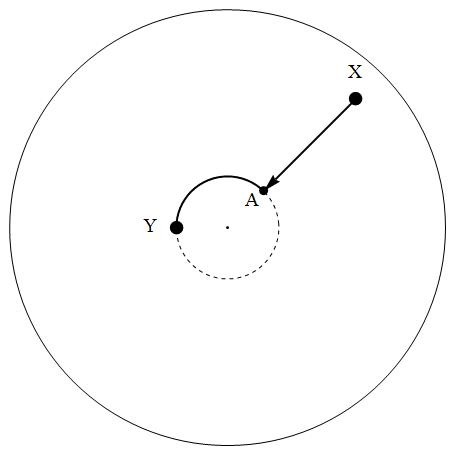
\includegraphics[width=0.25\textwidth]{figures/ShortArcStrategy.jpg}
\end{center}

Bardziej elastyczny sposób polega na otoczeniu grafiki konstrukcją \texttt{picture} (patrz Rys. \cref{fig:Lines}).
Poniżej znajduje się \cref{fig:Lines}. \par
Szablon pracy dyplomowej wykorzystuje pakiet \texttt{cleveref}. Służy on do elastycznego operowania referencjami wewnątrz dokumentu.  Na przykład, używając komendy \texttt{cref} (zamiast standardowej \verb|\ref{fig:Lines}|), 
nie musisz samemu pisać skrótu \texttt{Rys.}

\begin{figure}[ht]
  \centering
  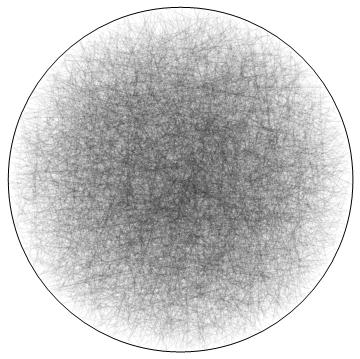
\includegraphics[scale=0.45]{figures/RandomLines.jpg}
  \caption{Symulacje 10000 losowych odcinków w kółku jednostkowym. Rysunek został samodzielnie wygenerowany.}
	\label{fig:Lines}
\end{figure}

Jeśli odkomentujesz polecenie \verb|\listoffigures| w głównym pliku, 
to rysunek ten znajdzie się na wygenerowanej liście rysunków.

\section{Wzory matematyczne}

Wzory matematyczne w obrębie paragrafu formatuje się za pomocą polecenia 
\verb|$ ... $|, np. $f(x) = \sin(x^2)$.
Za pomocą polecenia \verb|\[ ... \]| formatujesz równania wycentrowane bez numerowania, np.
\[
  \sin^2(\alpha) + \cos^2(\alpha) = 1 ~,
\]
a za pomocą konstrukcji \verb|\begin{equation} ... \end{equation}| 
formatujesz równania numerowane, np.
\begin{equation} \label{eq:ExpFnc}
 \exp(I \cdot t) = \cos(t) + I\cdot\sin(t)
\end{equation}
Równań numerowanych używaj \textbf{tylko wtedy}, gdy będziesz się do nich odwoływać w dalszej części tekstu 
za pomocą polecenia \verb|\ref{...}|.  

Jeśli w pracy znajdą się jakieś twierdzenia, lematy, to skorzystaj z konstrukcji \texttt{theorem}, \texttt{lemma}, \texttt{corollary}   oraz \texttt{proof}, zdefiniowanych w pakiecie \texttt{amsthm}, zaimportowanym do tego szablonu. Oto przykład:

\begin{theorem}[Euklides]
Istnieje nieskończenie wiele liczb pierwszych.
\end{theorem}

\begin{proof} 
Załóżmy, że $p_1,\ldots,p_n$ jest listą wszystkich liczb pierwszych. Niech
\[
  q = (p_1\cdot\cdots\cdot p_n) + 1 ~.
\]
Wtedy $q>1$, istnieć więc musi liczba pierwsza $p$ taka, że $p|q$. ...
\end{proof}

\section{Cytowania}
\label{examples:cite}

W tym szablonie korzystamy z biblioteki \texttt{biber} do formatowania cytatów. 
Jest to nowocześniejsza wersja standardowej (ale obecnie już nie rozwijanej) biblioteki \texttt{bibtex}.
Oto przykład użycia:

\begin{quote}
   Książka \cite{KNUTH01} jest poświęcona podstawowym algorytmom. 
   Autor \citeauthor{KNUTH01} omawia w niej większość klasycznych algorytmów. 
   Z punktu widzenia tej pracy ważny jest algorytm znajdujący się w \textcite[249]{KNUTH02}.\par
   Prace \cite{KuhnWZ08}, \cite{PapaGeo07} zawierają zwięzłe wprowadzenia do problematyki \textit{routingu geograficznego}.
\end{quote}

Wpisy opisujące źródła bibliograficzne najlepiej jest przechowywać w oddzielnym pliku o formacie \texttt{bibtex}. 
Do szablonu dołączony jest przykładowy plik \texttt{bibliography.bib}. Znajdują się w nim przykłady podstawowych typów tzw. wpisów.
Porządnie sformatowane wpisy bibliograficzne możesz znaleźć, na przykład, na stronach 
\href{https://dblp.org/}{dblp} oraz w serwisie \href{https://scholar.google.com/}{Google Scholar}. \par


Biber, używany z pakietem biblatex, zapewnia wiele predefiniowanych stylów formatowania cytatów i bibliografii, z typowymi stylami takimi jak  
\texttt{numeric}, \texttt{alphabetic}, \texttt{authoryear}, \texttt{authortitle} i \texttt{verbatim}, 
wraz z opcjami sortowania, takimi jak \texttt{nty} (name, title, year) lub \texttt{nyt} (name, year, title). 
Style te są wybierane za pomocą opcji \texttt{style=} w poleceniu 
\begin{center}
\verb|\usepackage[backend=biber, style=...]{biblatex}| 
\end{center}
w preambule Latex'a. Stosowany w pracy styl formatowania ustal wspólnie z opiekunem pracy. W pliku \texttt{main.tex} zaproponowano styl numeryczny bez opcji sortowania, co oznacza, że bibliografia będzie wyświetlana w kolejności pojawienia się cytowanej pozycji w tekście pracy. 

\subsection*{Uwaga} Cytowania w Latex'u możesz samodzielnie obsługiwać bez pomocy pliku w formacie bibtex. Jednak samodzielne, poprawne sformatowanie bibliografii jest dość żmudne. Pamiętaj również o tym, że każda pozycja występująca w spisie literatury musi być cytowana w tekście pracy.  

\section{Tabele}

Tabele wstawiasz w sposób standardowy. 
Po odkomentowaniu polecenia  \verb|\listoftables| z głównego pliku tego szablonu do pliku zostanie dołączona lista tabel.
Do tej tabeli możesz się odwoływać za pomocą polecenia \verb|\cref{tab:example}| (\cref{tab:example}).
                                             
\begin{table}[htbp]
  \caption{Przykładowa tabela }
  \centering
  \begin{tabular}{|l|l|r|}
    \hline
    \textbf{Kategoria} & \textbf{Parametr} & \textbf{Wynik} \\
    \hline
    Test A & Niskie obciążenie & 15 ms \\
    Test B & Wysokie obciążenie & 120 ms \\
    \hline
  \end{tabular}
  \label{tab:example}
\end{table}

\section{Kody procedur}

Do tego szablonu dołączony został pakiet \texttt{listings}. 
Ułatwia on wstawianie kodów źródłowych do dokumentu. W szablonie, w pliku \texttt{ustawienia.tex},  
są ustawione domyślne parametry wyświetlania dla kodów. 

Oto przykład jego użycia:

\begin{lstlisting}[language=C, 
caption={Algorytm Euklidesa w języku C}, 
label={lst:hello}]
/* 
 * Algorytm Euklidesa.
 * Zwraca gcd(a, b).
 */
int gcd(int a, int b)
{
    while (b != 0) {
        int r = a % b;
        a = b;
        b = r;
    }
    return a;
}
\end{lstlisting}

Oto inny przykład, kod implementacji algorytmu QuickSort w języku Haskell (\cref{lst:hhaskell:qs}) wykorzystujący,
dla zwiększenia czytelności kodu,  mechanizm \textit{list comprehension}: \par

\begin{lstlisting}[style=haskellStyle, %language=haskell, 
caption={Algorytm QuickSort w języku Haskell}, 
label={lst:hhaskell:qs}]
-- QuickSort: czas O(n^2); średni czas O(n log(n))
qs [] = []
qs (x:xs) = qs [t| t<- xs, t < x] ++ 
            [x] ++ 
						qs [t| t<- xs, t >= x]
\end{lstlisting}


Do wstawiania pseudokodów do pracy zalecamy korzystanie z pakietów \texttt{algorithm} oraz \texttt{algpseudocode} dołączonych do tego szablonu.
Oto przykład pseudokodu zapisanego w języku tych pakietów (\cref{ps:filtr}):


\begin{algorithm}[H]
\caption{Filtrowanie}
\label{ps:filtr}
\begin{algorithmic}[1]
\State Initialize: $S \gets \emptyset$
\For{$v \in V$}
  \If{$\mathrm{condition}(v)$}
    \State $S \gets S \cup \{v\}$ \Comment{Dodaj jeśli spełnia warunek}
  \EndIf
\EndFor
\State \Return $S$
\end{algorithmic}
\end{algorithm}

\section{Akronimy}

Szablon ten korzysta z pakietu \texttt{acro}. Plik \texttt{acronims.tex} jest przykładem pliku konfiguracyjnego.
Oto przykład użycia:
\begin{quote}
  Podczas budowania oprogramowania dużą wagę przykładaliśmy do przestrzegania dwóch 
	zasad: zasady \ac{dry} oraz zasady \ac{kiss} 
\end{quote}
Za drugim razem, gdy użyjesz synonimów, pojawią się już tylko skrócone nazwy, na przykład:
\begin{quote}
  Stosowanie zasady \ac{dry} polega unikaniu pisania kilkukrotnie podobnych fragmentów kodu.  Stosowanie tej zasady znacznie ułatwia modyfikację kodów. 
  Z kolei stosowanie zasady \ac{kiss} zmusza programistę do systematycznego zastanawiania się nad jakością swojego kodu.
\end{quote}

Jeśli nie masz potrzeby korzystania z akronimów, to zakomentuj dwie linie w pliku \texttt{main.tex} (linie 59 oraz 73).
 
 %% Tu jest kilka przykładów

%% TU WYWOŁUJEMY BIBLIOGRAFIĘ
%% ZRÓDŁO ZOSTAŁO USTAWIONE POLECENIEM \addbibresource
%% W NAGŁÓWKU STRONY
%\printbibliography[heading=bibintoc, title={Spis literatury}]
\printbibliography[title={Spis literatury}]
%% TU ZACZYNAJĄ SIĘ ZAŁĄCZNIKI
\appendix
%% \include{Dodatek01}
%% ...
%% \include{DodatekYY}


%% --- Spisy ---
%% odkomentuj potrzebne spisy 
%% (zastanów się, czy są Ci one potrzebne)
 
%\listoffigures
%\listoftables
%\lstlistoflistings

\end{document}